\documentclass[a4paper,12pt]{article}
\usepackage{natbib,epsfig,rotating}

\title{Visualisation of SPH data using SUPERSPHPLOT - v1.0}
\author{Daniel Price}

\begin{document}
\maketitle
\tableofcontents

\newpage
\section{Introduction}
SUPERSPHPLOT is a utility for visualisation of output from (astrophysical) simulations using the
Smoothed Particle Hydrodynamics (SPH) method in one, two and three dimensions. It is written entirely in Fortran 90 and
utilises PGPLOT subroutines to do the actual plotting. In particular the following
features are included:
\begin{itemize}
\item Rendering of particle data to an array of pixels using the SPH kernel
\item Cross-sections through 2D and 3D data (as both particle plots and rendered
images).
\item Fast projections through 3D data (ie. column density plots, or integration of
other quantities along the line of sight)
\item Vector plots of the velocity (and other vector quantities), including vector
plots in a cross section slice in 3D.
\item Rotation and fly-throughs (multiple cross-section slices) of 3D data.
\item Automatic stepping through timesteps, making animations simple to produce.
\item Interactive mode for detailed examination of timestep data (e.g. plotting
particle labels, working out the gradient of a line, stepping forwards/backwards
through timesteps)
\item Multiple plots on page, including option to automatically tile plots if $y-$ and $x-$ limits
are the same.
\item Plot limits can be fixed, adaptive or particle tracking. Also simple to change
axes to log, invert, square root or absolute of a quantity.
\item Exact solutions for common SPH test problems (e.g. hydrodynamic shock tubes,
polytropes).
\item Calculation of quantities not dumped (e.g. pressure)
\item Transformation to different co-ordinate systems (for both co-ordinates and
vector components).
\item Straightforward production of GIF and Postscript images.
\end{itemize}

\subsection{Why should I use it?}
 Whilst many wonderful commercial software packages exist for visualising scientific
data (such as the widely used Interactive Data Language), I found that such packages
could be somewhat cumbersome for the manipulation and visualisation of my SPH data. The
main problem was that much of what I wanted to do was fairly specific to SPH (such as
interpolation to an array of pixels using the kernel) and whilst generic routines exist
for such tasks, I could not explain how they worked, nor were they
particularly fast and nor could I incorporate into them my existing programs for doing
other things (such as the calculation of exact solutions). In fact, the major
work in the visualisation of SPH data is not the image production itself but the
manipulation of data prior to plotting. Much of this manipulation makes sense
within an SPH framework (for example the interpolation provided by the kernel
and rotation of the particles for perspective) and this is what this program is
designed to do - to use SPH tools to analyse SPH data and to make this a
straightforward task such that publishable images and animations can be obtained
as efficiently as possible from the raw data with a minimum amount of effort
from the user. I have found in the process that the development of powerful
visualisation tools has enabled me to pick up on effects present in my
simulation results that I would not otherwise have noticed (in particular the
difference between a raw particle plot and a rendered image can be substantial).

\subsection{Version History}
 This is the pre-public-release (Guinea-pig) version.

\section{Gallery}

\begin{figure}
\begin{center}
\begin{turn}{270}\epsfig{file=hyperbolic.ps,height=\textwidth}\end{turn}
\label{fig:hyperbolic}
\end{center}
\end{figure}

\section{Getting started}
 First of all, make sure that PGPLOT is installed on your system. The PGPLOT
graphics subroutine library is freely downloadable from
\begin{verbatim}
http://www.astro.caltech.edu/~tjp/pgplot/
\end{verbatim}
or by ftp from 
\begin{verbatim} 
ftp://ftp.astro.caltech.edu/pub/pgplot/pgplot5.2.tar.gz
\end{verbatim}
however check to see if it is already installed on your system (if so, the libraries are
usually located in /usr/local/pgplot). For details of the actual plotting subroutines
used by SUPERSPHPLOT, we refer the reader to the PGPLOT userguide:
\begin{verbatim}
http://www.astro.caltech.edu/~tjp/pgplot/contents.html
\end{verbatim}

\subsection{Compiling the code: Makefile options} 
 In the Makefile, you will need to set the FORTRAN compiler and flags to your local version, e.g..
\begin{verbatim}
F90C = f95
F90FLAGS = -O
\end{verbatim}
 Secondly the compiler must be able to link to the PGPLOT and X11 libraries on
your system. As a first attempt try using:
\begin{verbatim}
LDFLAGS = -lpgplot -lX11
\end{verbatim}
If that works at a first attempt, take a moment to think several happy thoughts about your system
administrator. If these libraries are not found, you will need to enter the
library paths by hand. On most systems this is something like:
\begin{verbatim}
LDFLAGS = -L/usr/local/pgplot -lpgplot -L/usr/X11R6/lib -lX11
\end{verbatim}
(assuming the PGPLOT libraries are in the /usr/local/pgplot directory and the
X11 libraries are in /usr/X11R6/lib). If, having found the PGPLOT and X11
libraries, the program still won't compile, it is usually
because the PGPLOT on your system has been compiled with a different compiler to
the one you are using. A first attempt is to try using the g2c libraries
\begin{verbatim}
LDFLAGS = -L/usr/local/pgplot -lpgplot -L/usr/X11R6/lib -lX11 -lg2c
\end{verbatim}
On some systems I have also had to use
\begin{verbatim}
LDFLAGS = -L/usr/local/pgplot -lpgplot -L/usr/X11R6/lib -lX11 -lg2c -lpng
\end{verbatim}
Failing that, ask your system administrator!!

\subsection{Environment variables}
 Several useful environment variables can be set for PGPLOT and several of them
are very useful for SUPERSPHPLOT. In a tcsh shell type:
\begin{verbatim}
setenv PGPLOT_DEV /xwin
setenv PGPLOT_BACKGROUND white
setenv PGPLOT_FOREGROUND black
\end{verbatim}
The first command sets the default device to the X-window, rather than the /null
device. The latter two commands set the background and foreground colours of the
plotting page. Note that these environment variables should be set \emph{before}
invoking supersphplot (it is simplest to set them upon starting the shell by placing
them in your .tcshrc or bash/sh equivalent file). For other environment
variables which can be set, refer to the PGPLOT user guide.

\subsection{System dependent routines}
The only system dependent subroutine is the call to $getarg$ in supersphplot.f90 which
reads the run name(s) from the command line. A standardised format for performing this
task is included in the standards for the next release of Fortran (Fortran 2003),
however in the meantime this call may require some adjustment depending on the
particular system you are compiling the code on. The program is still fully
functional without this call working, but it does make things convenient.

\section{Reading data}

\subsection{Using the subroutines provided}
 The data format is specified in the subroutine read\_data.  
The filename is input on the command line, ie.
\begin{verbatim}
supersphplot myrun
\end{verbatim}
With multiple filenames on the command line, ie.
\begin{verbatim}
supersphplot myrun1 myrun2 myrun3
\end{verbatim}
or simply
\begin{verbatim}
supersphplot myrun*
\end{verbatim}
files will be read consecutively in the order that they are given.

\subsection{Writing your own subroutine}
The first $ndim$ columns in the main data array \emph{must} contain the particle co-ordinates.
Also it is preferable (but not essential) for the next $ndimV$ columns to contain the
particle velocities (note that the co-ordinates and velocities can in general have different
numbers of dimensions since this can occur, for example, in MHD simulations). After
these columns the ordering of data is not important, although vector quantities should
always be listed with components in the correct order (e.g. $(\nabla\times {\bf v})_x$,
followed by the $y-$ and $z-$ components) for both vector plotting and the co-ordinate
transformation of the vector quantities. 

Most important is that, for the rendering routines to work, the density, particle
masses and smoothing lengths for \emph{all} of the (gas) particles \emph{must} be read in from
the data file and their locations in the main data array labelled using the global
parameters $irho, ipmass$ and $ih$. Labelling of the location of other particle
quantities (e.g. $iutherm$ for the thermal energy) is used in
order to plot the exact solutions on the appropriate graphs and also for calculating
additional quantities (e.g. calculation of the pressure uses $iutherm$ and $irho$).

\section{Program structure}

defaults\_read

get\_data

set\_kerneltables

calc\_quantities

limits\_set

menu

main plotting loop

options

\subsection{Modules}

\subsection{Subroutines}
The program consists of the following subroutines (in alphabetical order):
\begin{tabular}{lcp{0.7\textwidth}}
allocate           & : & allocates memory for main arrays \\
calc\_quantities    & : & calculates additional quantities from particle data\\
colour\_demo        & : & demonstration of colour schemes for rendering\\
colour\_set	 & : & sets up pgplot colour table for rendering\\
coord\_transform    & : & transforms between various coord systems\\
danpgsch           & : & sets character height independent of page size\\
danpgtile          & : & my utility for tiling plots on the pgplot page\\
danpgwedg          & : & my very minor modification of pgwedg\\
defaults\_read	 & : & read default plot options from file\\
defaults\_set	 & : & sets default plot options if not read from file\\
defaults\_write	 & : & write default plot options to file\\
exact\_fromfile     & : & reads an exact solution tabulated in a file\\
exact\_mhdshock     & : & some tabulated solutions for mhd shocks \\
exact\_polytrope    & : & exact solution for a polytrope\\
exact\_rhoh	 & : & plots exact relation between density and smoothing length\\
exact\_sedov        & : & exact solution for sedov blast wave\\
exact\_shock        & : & exact solution for hydrodynamic shocks\\
exact\_swave        & : & exact solution for a linear sound wave\\
exact\_toystar      & : & exact solution for the toy star problem\\
get\_data           & : & wrapper for main data read\\
interactive\_part   & : & interactive utilities for particle plots\\
interpolate1D	 & : & interpolation of 1D sph data to 1D grid using sph kernel\\
interpolate2D	 & : & interpolation of 2D sph data to 2D grid using sph kernel  \\   
interpolate2D\_xsec & : & oblique 1D cross section through 2D sph data using kernel\\
interpolate3D	 & : & interpolation of 3D sph data to 3D grid using sph kernel\\
interpolate3D\_fastxsec   & : & fast cross section through 3D data using sph kernel\\
interpolate3D\_projection & : & fast projection of 3D data to 2D grid using integrated sph kernel\\
interpolate3D\_xsec\_vec   & : & fast cross section of vector quantity in 3D data using kernel\\
legend		       & : & plots legend on plot (time)\\
limits\_read              & : & reads plot limits from file\\
limits\_save              & : & saves plot limits to file\\
limits\_set               & : & calculates plot limits\\
main               & : & main plotting loop\\
menu               & : & main menu\\
modules		 & : & contains all shared (global) variables\\
options\_data       & : & sets options relating to current data\\
options\_exact	 & : & sets options and params for exact solution calculation/plotting\\
options\_limits     & : & sets options relating to plot limits\\
options\_page       & : & sets options relating to page setup\\
options\_particleplots & : & sets options relating to particle plots\\
options\_powerspec  & : & sets options for power spectrum plotting\\
options\_render	 & : & sets options for render plots\\
options\_vector	 & : & sets options for vector plots\\
plot\_average	 & : & bins particles along x-axis and plots average line\\
plot\_kernel\_gr     & : & plots the kernel shape in non-cartesian co-ordinates\\
plot\_powerspectrum & : & calls powerspectrum and plots it\\
powerspectrum\_fourier & : & calculates power spectrum of 1D data on ordered pts\\
powerspectrum\_lomb & : & calculates power spectrum of 1D data on disordered pts\\
read\_data\_dansph   & : & reads data from my format of data files\\
read\_data\_mrbsph   & : & reads data from matthew bate's format of data files\\
render	 	 & : & takes array of pixels and plots render map/contours etc\\
riemannsolver      & : & Riemann solver (called by exact\_shock)\\
setpage            & : & sets up the PGPLOT page (replaces call to PGENV/PGLAB)\\
supersphplot	 & : & main program, drives menu loop\\
titles\_read        & : & reads a list of titles to be used to label each timestep\\
transform	 	 & : & applies various transformations to data (log10, 1/x, etc)\\
vectorplot         & : & produces a vector plot from particle data
\end{tabular}

\subsection{Variables}
\label{sec:variables}

\section{Options}
 The program options may be changed in a series of submenus. The defaults for all of
these options are initially set in the subroutine defaults\_set. The options set using
the submenus can be saved using the (s)ave option from the menu. This saves all of
the current options to a file called `defaults' in the current directory, which is
automatically read upon starting supersphplot the next time. This file is written using
the namelist formatting option provided by Fortran 90. An alternative way of setting
options is to edit this file directly prior to invoking the program, referring to the
variable list given in \S\ref{sec:variables} of this user guide. 

\subsection{(m)ultiplot}

\subsection{(d)ata options}
These options relate to the data read and are as follows:
\begin{enumerate}
\item \textbf{read new data}. Read new data, using a different runname.
\item \textbf{change number of timesteps read}. Set timestep number to start
reading from, timestep number to stop reading from and the frequency of
timesteps to read (e.g. every two steps). This can also be changed interactively in
interactive mode.
\end{enumerate}

\subsection{(i)nteractive mode}
 The menu option turns on/off interactive mode. With this option turned on and
an appropriate device selected (ie. the X-window, not /gif or /ps), after
each plot the program waits for specific commands from the user. With the cursor
positioned anywhere in the plot window, commands can be invoked using the
following keystrokes:

\begin{tabular}{rcp{0.75\textwidth}}
 h & : & display/hide help text \\
 p & : & label the particle closest to the cursor position \\
 l & : & draw a connecting line between the closest particle and a second
 particle (to be selected) and calculate the slope of this line. \\
 r & : & replot the current plot. \\
 left click & : & advance to next timestep \\
 right click & : & go back to previous timestep \\
  1,2,3..9 & : & on click, jump forward/backwards by $n$ timesteps \\
  q & : & quit plotting 
\end{tabular}

 NB: If the multiplot option has been used, the timestep changing commands only
take effect on the last plot per timestep. Many more commands could be added to
the interactive mode, limited only by your imagination. Please send me your suggestions!

\subsection{(p)age options}
 This submenu contains options relating to the PGPLOT page setup. The options are as follows:
\begin{enumerate}
\item \textbf{toggle page change}. (default=on) When turned off, no new page is
created between plots. This means that consecutive timesteps are plotted
directly on top of one another. For particle plots this can be used to trace the
position of the particles as they evolve in time.
\item \textbf{toggle axes}. Changes the appearance of the axes. The variable is
the same as the AXIS variable used in the call to PGENV in the standard PGPLOT
routines, except that I have also added the $-3$ option. The options are
as follows:

\begin{tabular}{rcp{0.8\textwidth}}
-3 & : & same as AXIS=-1, but also draw tick marks; \\
 -2 & : & draw no box, axes or labels; \\
 -1 & : & draw box only; \\
  0 & : & draw box and label it with coordinates; \\
  1 & : & same as AXIS=0, but also draw the coordinate axes (X=0, Y=0); \\
  2 & : & same as AXIS=1, but also draw grid lines at major increments of the coordinates;
\end{tabular}

\item \textbf{change paper size}. Sets the size of the plotting page.
\item \textbf{change plots per page}. Changes the number of plots on each
physical page.
\item \textbf{toggle plot tiling}. When set, plots with more than one plot on
the page and the same $y-$ and $x-$ axes are automatically tiled together.
\item \textbf{adjust title position}. Adjusts the position of the title on
each plot.
\item \textbf{adjust legend position}. Adjusts the position of the legend on
each plot.
\item \textbf{toggle animate}. When set, this turns off the prompting given
before the page is changed. Does not apply in interactive mode, where the page
changing can be controlled using the mouse. 
\end{enumerate}

\subsection{particle plot (o)ptions}
 These options relate to pure `particle plots'. The options are as follows:
\begin{enumerate}
\item \textbf{toggle plot line}. When set, this option plots a line connecting the particles
in the order that they appear in the data array. Useful mainly in one dimension, although can give an indication of the
relative closeness of the particles in memory and in physical space in higher dimensions.
\item \textbf{toggle plot average line}. Bins the particles into $nbin$ bins along the
$x-$axis, calculates the average value of the $y-$axis quantity in each bin and
plots a line through these points. 
\item \textbf{toggle label particles}. This option prints the number of each particle
next to its position on the plot (for all particles). Primarily useful for debugging neighbour finding
routines. An alternative is to use the `p' option in interactive mode.
\item \textbf{circles of interaction}. On coordinate plots this option plots a circle of
radius $2h$ around either all particles or on up to 10 selected individual particles. 
This is primarily useful in debugging neighbour finding routines. On
non-coordinate plots an error bar of length $2h$ in either direction is plotted
in the direction of the coordinate axis.
\item \textbf{plot ghosts/sinks}. Enables particles of certain types only to be plotted
(e.g. dark matter particles only, gas particles only or both).
\item \textbf{change graph markers}. This option sets the PGPLOT marker used for each
type of particle in the particle plots. The list of markers is given in the
PGPLOT user guide and is also listed in Appendix \ref{sec:pgplotmarkers}. 
\item \textbf{toggle cross section/projection}. In three dimensions this determines
whether to all the particles projected onto the plane or to plot particles only
in a given co-ordinate range. Also applies to rendered and vector plots.
\item \textbf{change co-ordinate systems}. This feature transforms the particle
co-ordinates and vector components into non-cartesian co-ordinate systems. This
is useful for simulation data which has a particular symmetry associated with it
(e.g. for accretion disc simulations, the components of velocity in the radial
and azimuthal directions can be plotted). Note that this option does \emph{not} change
the co-ordinate system used on rendered plots, as this would mean that the interpolation using the SPH
kernel would not be correct.  
\item \textbf{toggle exact solution}. The following exact solutions are provided
\begin{itemize}
\item Hydrodynamic shock tubes (Riemann problem)
\item Spherically-symmetric sedov blast wave problem. This
\item Polytropes (with arbitrary $\gamma$)
\item One dimensional toy stars. This is a particularly simple test
problem for SPH codes described in \citet{mp04}.
\item Linear wave. This simply plots a sine wave of a specified amplitude, period and
wavelength on the plot specified.
\item MHD shock tubes (tabulated). These are tabulated solutions for 7 specific MHD
shock tube problems.
\item Exact solution from a file. This option reads in an exact solution from the
filename input by the user, assuming the file contains two columns containing the $x-$ and $y-$ co-ordinates of
an exact solution to be plotted as a line on the plot specified.
\end{itemize}
Details of the calculation of the exact solutions and examples of their output are
given in Appendix \ref{sec:exact}. Note that the PGPLOT call to plot the line is included in the
exact solution subroutine so as to provide flexibility should an exact solution require
multiple lines on the page / different line styles etc. (although none of those
provided do).
\end{enumerate}


\subsection{plot (l)imits}
 The options for plot limits are as follows:
\begin{enumerate}
\item \textbf{toggle fixed/adaptive limits}. With limits set to adaptive, plot
limits are minimum and maximum of quantities at current
timestep. However, the co-ordinate limits are not adapted in the case of
rendered plots. With fixed limits, the plot limits retain their default values
for all timesteps.
\item \textbf{set manual limits}. Manually set the limits for each column of
data.
\item \textbf{x-y limits track particle}. Co-ordinate limits are centred on the
selected particle for all timesteps, with offsets as input by the user. This
effectively gives the `Lagrangian' perspective.
\item \textbf{zoom in/out}.
\item \textbf{apply transformations (log10,1/x)}.
\item \textbf{save current limits to file}. Saves the current values of the
limits calculated from the data read or set manually using option (2) to the
file `rootname.limits' where rootname is the name of the current run. This file
is automatically read upon the next invocation of supersphplot. The limits apply
only when fixed limits are set.
\item \textbf{re-read limits file}. Re-reads the plot limits from the
`rootname.limits' file. This means that the limits contained in this file can be
manually changed by the user whilst the program is still running.
\end{enumerate}

\subsection{(r)endering options}
\begin{enumerate}
\item \textbf{change number of pixels}. Set the number of pixels along the
$x-$axis. Pixels are assumed to be square such that the number of pixels along
the $y-$axis is determined by the aspect ratio of the current plot.
\item \textbf{change colour scheme}. Changes the colour scheme used on rendered
images. A demonstration of all the colour schemes can be also be invoked from
this menu option. Setting the colour scheme to zero plots only the contours of
the rendered quantity (assuming that plot contours is set to true). The colour
schemes given are as follows:

\begin{tabular}{rcp{0.8\textwidth}}
  0 & : & contours only \\
  1 & : & greyscale \\
  2 & : & red \\
  3 & : & ice blue \\
  4 & : & rainbow \\
  5 & : & frog monster
\end{tabular}

User contributed colour schemes are eagerly invited (see the subroutine
`colour\_set' for details on how to do this).
\item \textbf{toggle cross section/projection}. For 3D data, toggles whether to
plot the rendered quantity integrated along the line of sight (projection) or in
a particular cross section along the line of sight. For 2D data setting the
cross section option gives arbitrary 1D cross sections through 2D data. Also applies to vector and plots.
\item \textbf{toggle plot contours}. Determines whether or not to plot contours
in addition to the rendered quantity.
\item \textbf{change number of contours}. Sets the number of contours to be
plotted. 
\item \textbf{toggle colour bar}. Determines whether or not to plot the colour
bar on rendered images.
\end{enumerate}

\subsection{(v)ector plot options}
\begin{enumerate}
\item \textbf{change number of pixels}. Set the number of pixels along the
$x-$axis to be used in the vector plots. As in the rendered images, pixels are assumed to be square such that the number of pixels along
the $y-$axis is determined by the aspect ratio of the current plot.
\item \textbf{toggle particle plotting if no rendering}. If no rendered quantity
is set, toggles whether or not to plot the particles in addition to the vector
plot.
\item \textbf{toggle background/foreground colour}. Determines whether or not to
plot the vector arrows in the current background or foreground colour (by
default these are white and black respectively). This must
be user determined to give the best contrast between the vector arrows and the
rendered image.
\end{enumerate}

\subsection{(s)ave, (h)elp, (q)uit}
 The (s)ave options saves the default options to a file called `defaults' in the
current directory which is read automatically upon the next invocation of
supersphplot. The (h)elp option simply expands the text for the options menus (I
may add to this soon). (q)uit, unsurprisingly, quits. Typing a number greater than the number of
data columns also exits the program (e.g. I often simply type 99 to exit).

\section{The guts}

\subsection{Rendering/contour plots}
 For a contour or rendered plot of a scalar quantity $\phi$ we
interpolate from the particles to an array of pixels using the SPH summation
interpolant.

In two dimensions the interpolant is simply
\begin{equation}
\phi(x,y) = \sum_b m_b \frac{\phi_b}{\rho_b} W(x - x_b, y-y_b, h_b)
\end{equation}
where $W$ is the usual cubic spline kernel and the summation is over
contributing particles.

In three dimensions, we must either take a cross section or a projection
through the data.

\subsection{Cross sections}

\subsubsection{Cross sections of 3D data}
 A cross section can be taken of SPH data by summing the
contributions to each pixel in the cross section plane from all particles within
$2h$ of the plane. This is done in the subroutine interpolate\_3D\_fastxsec. In
this case the cross section is always at a fixed value of the third co-ordinate
(ie. for xy plots the cross section is in the z direction). Oblique cross
sections can be taken by rotating the particles first.

 A routine is also provided to do cross sections of two dimensional data (ie. take one dimensional
cross sections) (interpolate2D\_xsec). In this case the cross-section line can be arbitrarily
specified. I will hopefully write an interactive version of this one day.

\subsubsection{Cross sections of 2D data}
The cross-sectioning algorithm for 2D data (giving a 1D line) is slightly
different, in that it also works for oblique cross sections. The
cross-sectioning is done in the subroutine interpolate2D\_xsec. The cross
section is defined by two points (x1,y1) and (x2,y2) through which the line
should pass. These points are converted to give the equation of the line in the
form
\begin{equation}
y = mx + c
\end{equation}
This line is then divided evenly into pixels to which the particles
may contribute. The contributions along this line from the particles is computed
as follows: 

 For each particle, the points at which the cross section line intersects the
smoothing circle are calculated (illustrated in Figure \ref{fig:xsec2D}). The
smoothing circle of particle $i$ is defined by the equation
\begin{equation}
(x-x_i)^2 + (y-y_i)^2 = (2h)^2
\end{equation}
The x-coordinates of the points of intersection are the solutions to the quadratic equation
\begin{equation}
(1 + m^2) x^2 + 2 (m (c - y_i) - x_i) x + (x_i^2 + y_i^2 - 2cy_i + c^2 - (2h)^2)= 0
\end{equation}
For particles which do not contribute to the cross section line, the determinant
is negative. For the particles that do, it is then a simple matter of looping
over the pixels which lie between the two points of intersection, calculating
the contribution using the SPH summation interpolant
\begin{equation}
\phi = \sum_b m_b \frac{\phi_b}{\rho_b} W(x - x_b, h_b)
\end{equation}

\begin{figure}
\begin{center}
%%\begin{turn}{270}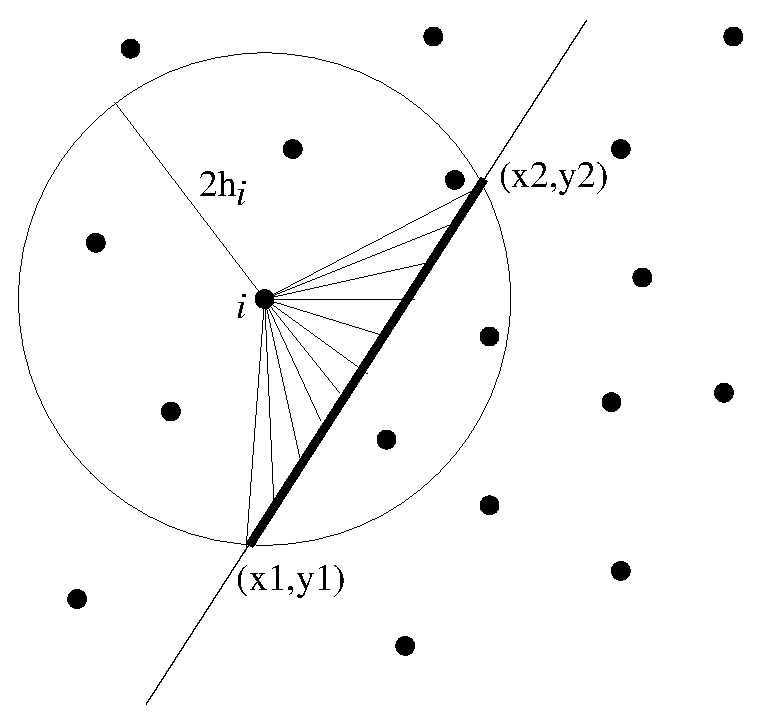
\epsfig{file=xsec2D.ps,height=\textwidth}\end{turn}
\label{fig:xsec2D}
\end{center}
\end{figure}
 
 An example of a 1D cross section through 2D data is shown in Figure
\ref{fig:xsec2Dexample}.
\begin{figure}
\begin{center}
%%\begin{turn}{270}\epsfig{file=xsec2Dexample.ps,height=\textwidth}\end{turn}
\label{fig:xsec2Dexample}
\end{center}
\end{figure}

 In principle a similar method could be used for oblique cross sections
through 3D data. In this case we would need to find the intersection
between the smoothing sphere and the cross section plane. However
in 3D it is simpler just to rotate the particles first and then take
a straight cross section as described above.
\subsection{Projections}


\subsection{Vector plots}

\subsection{Rotation}


\subsection{Co-ordinate transformations}



\section{FAQS: How do I...?}

\subsection{Read/process my data into images without having to answer prompts}

\subsection{Calculate additional quantities}

\subsection{Title the plots}

\subsection{Customise the legend}

\subsection{Make movies}
 Although the 

\section{User contributions / Wishlist for future improvements}
 Please contribute!! Any user contributions and/or suggestions would be greatly
appreciated. The following in particular would be very useful:

\begin{itemize}
\item Exact solutions for your favourite test problem(s). It would be great to
build a library of user-contributed exact solutions.
\item Data analysis tools (e.g. fourier transforms / statistical analysis /
algorithms for finding binary stars etc) which could be incorporated.
\item New visualisation techniques (e.g. an isosurfacing routine for SPH, better
vortex line tracing).
\item Better colour schemes!!! (see colour\_set.f90 for how to do this)
\end{itemize}

If you wish to send me subroutines or snippets of (Fortran only!) code for doing any of the above or
more, please also send me a \LaTeX file
documenting the subroutine similar to the documentation given in this user guide.
Also, please, please comment your code clearly so that others can figure out
what it does and try to catch as many errors as possible so that the whole
program is robust.  One thing I have avoided doing is to use any specific SPH routines, so that I
don't have to use any treecodes or the like to find neighbours. An example of a
routine which would use this is to find the div/curl of a vector quantity using
the SPH summation.

Contributions, comments and inevitable bug fixes
should be sent to:
\begin{verbatim}
dprice@ast.cam.ac.uk
\end{verbatim}
although check that this email address is current because I am still a postdoc!


\section*{Acknowledgements}
 Several of the routines were developed from ideas used by Matthew Bate. The
polytrope exact solution is from a routine by Joe Monaghan. I am indebted to one
Thomas S. Ullrich at the University of Heidelberg who wrote the prompting module
which is used throughout the program.

\newpage
\appendix

\section{Exact solutions}
\label{sec:exact}
\subsection{Shock tubes (Riemann problem)}
 This subroutine plots the exact solution for a one-dimensional shock tube
(Riemann problem). The difficult bit of the problem is to determine the jump in
pressure and velocity across the shock front given the initial left and right
states. This is performed in a separate subroutine (riemannsolver) as there are 
many different methods by which this can be done (see e.g. \citealt{toro92}). 
The actual subroutine exact\_shock reconstructs the shock profile (consisting of
a rarefaction fan, contact discontinuity and shock, summarised in Figure
\ref{fig:shocktube}), given the post-shock values of pressure and
velocity. 

 The speed at which the shock travels into the `right' fluid can be computed from the post shock
velocity using the relation
\begin{equation}
v_{shock} = v_{post}\frac{(\rho_{post}/\rho_R)}{(\rho_{post}/\rho_R)- 1},
\end{equation}
where the jump conditions imply
\begin{equation}
\frac{\rho_{post}}{\rho_R} = \frac{(P_{post}/P_R) + \beta}{1 + \beta (P_{post}/P_R)}
\end{equation}
with
\begin{equation}
\beta = \frac{\gamma - 1}{\gamma + 1}.
\end{equation}

\subsubsection{Riemann solver}
 The algorithm for determining the post-shock velocity and pressure is taken
from \citet{vanleer79} (reprinted as \citealt{vanleer99}).


\subsection{Polytrope}
 This subroutines computes the exact solution for a static polytrope with
arbitrary $\gamma$.

\subsection{Linear wave}
 This subroutine simply plots a sine function on a given graph.

\subsection{Sedov blast wave}
 This subroutine computes the self-similar Sedov solution for a blast wave.

\subsection{Toy stars}
 See \citet{mp04}. The system is one dimensional with velocity $v$, density $\rho$, and pressure
$P$. The acceleration equation is 
\begin{equation}
\frac{dv}{dt} = - \frac{1}{\rho} \frac{\partial P}{\partial x}  - \Omega^2 x,
\end{equation}
 We assume the equation of state is 
\begin{equation}
P = K \rho^\gamma,
\end{equation} 

 The exact solutions provided assume the equations are scaled such that
$\Omega^2 = 1$.
 
\subsection{Static structure}
The static structure is given by
\begin{equation}
\bar \rho = 1- x^2,
\end{equation}

\subsection{Linear solutions}
The linear solution for the velocity is given by
\begin{equation}
v = 0.05 C_s G_n(x) \cos{\omega t} )
\end{equation}
density is
\begin{equation}
\rho = \bar{\rho} + \eta
\end{equation}
where 
\begin{equation}
\eta = 0.1 C_s \omega P_{n+1}(x) \sin{(\omega t)})
\end{equation}

\subsubsection{Non-linear solution}
In this case the velocity is given by
\begin{equation}
v = A(t) x,
\end{equation}
whilst the density solution is
\begin{equation}
\rho^{\gamma -1} = H(t) - C(t) x^2.
\end{equation}
where the parameters A, H and C are determined by solving the ordinary
differential equations
\begin{eqnarray}
\dot{H} & = & -AH(\gamma -1), \\
\dot{A} & = & \frac{2K \gamma}{\gamma -1} C - 1 - A^2 \\
\dot{C} & = & -AC(1+ \gamma),
\end{eqnarray}
The relation
\begin{equation}
A^2 = -1 - \frac{2 \sigma C}{\gamma -1} + kC^{\frac{2}{\gamma +1}},
\label{eq:kconst}
\end{equation}
is used to check the quality of the solution of the differential equations by
evaluating the constant $k$ (which should remain close to its initial value).

\subsection{MHD shock tubes}
 These are some tabulated solutions for specific MHD shock tube problems at a
given time taken from the tables given in \citet{dw94} and \citet{rj95}.

\subsection{h vs $\rho$}
 The subroutine exact\_hrho simply plots the relation between smoothing length
and density, ie.
\begin{equation}
h = h_{fact} \left(\frac{m}{\rho}\right)^{1/\nu}
\end{equation}
where $\nu$ is the number of spatial dimensions. The parameter $h_{fact}$ is
output by the code into the header of each timestep. For particles of different
masses, a different curve is plotted for each different mass value.

\newpage
\section{PGPLOT graph markers \& line styles}

\newpage

\bibliographystyle{klunamed}
\bibliography{/home/dprice/bibtex/sph,/home/dprice/bibtex/mhd}

\end{document}
